
\resetcounters

\markboth{Viallefond}{Formal Semantics to Model Experimental Data}

\title{Formal Semantics to Model Experimental Data}
\author{Fran\c{c}ois~Viallefond
\affil{LERMA, Observatoire de Paris, 61 av. de l'Observatoire 75014 Paris, France}}

\aindex{Viallefond, F.}

\begin{abstract}
The formalization of the Measurement Set reveals the ubiquity of a structure, a simplicial 2-complex. A subset of this complex is a hexagon encompassed into a triangle. The following shows that this hexagon also appears in the structure of the grammar of XML-Schema, a language used to express types or structures. This result gives insights to interpret this ubiquity. XML is famous for being described by itself (the schema of schema). Here we are in the case of models with this ubiquous structure which are described using a language with a grammar having itself that structure.
\end{abstract}

\section{Introduction}
Given the evolution of the instrumentation and the very large amount of data that they may produce, the role of a data model becomes critical. An attractive approach to model data is to transform the objects defined using our human language into mathematical objects thus leading to robust, efficient, and expressive data processors in information systems. Lets call the Measurement Set (MS) the model of the data acquired by telescopes in observatories. This model is shaped by action and operational semantics. We find that its overal structure is a simplicial 2-complex, its internal hexagonal pattern, a borromean structure. This structure appears to be ubiquitous in this approach.

The implementation of a model requires a modeling language. During the development of an application, {\it xsd2cpp}, which transforms models described using the XML-Schema language into C++ objects we find that this structure also organizes concepts defined in the XML-Schema grammar. The following presents this result and gives some insights for the interpretation. It borrows vocabulary from the XML-Schema W3C recommendation and the wsdlpull C++ schema processor. Due to limited space the detailed and complete study will be given elsewhere.

\section{Component and Uniqueness Constraints} 
When modeling an object or system, the semantic is captured by setting constraints. Let us consider an object defined by a tuple of elements. There is no element hierarchy. Let this tuple composed of parts, an {\it abstract} structure defined using grammar. Depending on how these parts are assembled there are two conceptual approaches:\\
{\it 1)} {\bf Type derivation}: this is the object oriented inheritance concept, the part being appended sequentially according to a type hierarchy. In type theory let the judgment $\Gamma \vdash A\!:\!Type$. The context $\Gamma$ is  a chain of arrows, $A_n\rightarrow A_{n-1}\rightarrow A\rightarrow ...\rightarrow A_0$. Constructing $A\!:\!type$ is a typed $\lambda$-calculus the $\lambda$ terms being the constructors of the $A_i ~\forall i\le n$. Note that the concept of multiple inheritance does not exist in XML-Schema.\\
{\it 2)} {\bf Composition}. In this case the components are composed according to a Component Model characterized by two things: {\it a) a model for the containment}: think of a component as a part in a partition. A part may be contained in the partition directly. Alternatively the containment is done by reference. In other words the definition of the part may be done either locally or at the global level, {\it b) a model of the component}. In that case there are 3 kinds, these identified by a {\it discriminator}, a member of the set $\{Particle,ParticleGroup, Container\}$. 

Note that these two approaches are not exclusive from each other, a technique often being used to set cohesion, i.e. structured semantic, by gluing the components using a common type hierarchy trunk.

\noindent
\begin{minipage}[h]{5.2cm}
Using the nomenclature of the schema processor, Figure~1 depicts the concept of a component: The syntactic terms are Id$_{group}$, the name, abstract, of a group defined at the global schema level, and Id$_{elem}$, the name of a particle, abstract iff substitutable else concrete. The dual is an anonymous container defined locally, a set of  elements (possibly a singleton), i.e. some kind of anonymous group or element. Underlying this diagram there are two inseparable concepts about the property of a component, two booleans: ``has name?'' and `has multiplicity?'' (there is multiplicity when the cardinality of the set of elements that a part may contain may
\end{minipage}
\begin{minipage}[h]{8.8cm}
 \begin{center}
 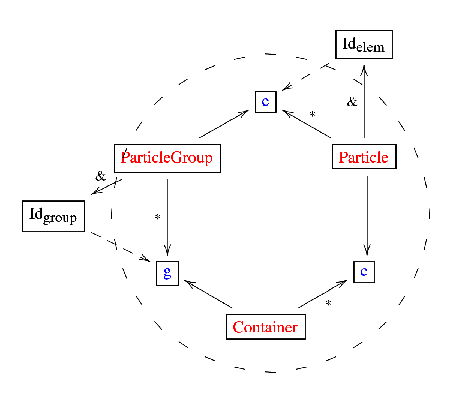
\includegraphics[]{part8/Viallefond_P52/P52_1.eps}
 \\Figure 1
 \end{center}

\end{minipage}
\hfill
be greater than one). Such a representation for a component is generic. Polymorphic it is fuzzy. Globally strict, it relies on the definition of this 
{\it discriminator}.


\section{Syntactic Term for a Uniqueness Constraint} 
The {\it xsd2cpp} converter generates regular types. A type is regular when
{\it a)} it is  {\it default constructible} which means that there is an initial object,
{\it b)} it is {\it assignable} i.e. there is a copy constructor and 
{\it c)} it has the concept of  {\it equality comparable} which implies identities and therefore there is at least one key. Think of a  key as a specific kind of part in a partition, the part and partition denoted respectively $Fields$ (the set of key fields) and \textit{Selector}. That pair is identified by a syntactic abstract term, the name of the key.
\noindent
\begin{minipage}[h]{5.2cm}
\indent
Any partition has a model of composition of its parts: the {\it compositor} parameter, a member of the set \{\textit{Choice, All, Sequence}\}. When a partition is a \textit{Selector}, if it has more than one part and if there is a single key then the model of composition has to be augmented by inference rules satisfying the normal forms of the relational model, the hypothesis made by  {\it xsd2cpp} when the schema processor finds keys.

Figure~2 depicts the concept of a generic type. Inside the circle is the {\it internal language} defining the Type. $Parts$ must be understood as the set of all the parts. Its dual is  $Partition$, the whole (the set of names {\it vs} the name of the set). 

\end{minipage}
\begin{minipage}[h]{8.8cm}
 \begin{center}

  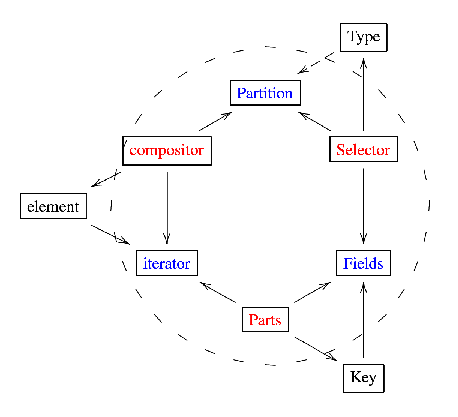
\includegraphics[]{part8/Viallefond_P52/P52_2.eps}
  \\Figure 2

 \end{center}
\end{minipage}
\hfill
\noindent
From the parts it is always possible to iterate linearly on them given the compositor parameter {\bf or} from the $Fields$ part to fork on the complementary parts (a set of accessors.) Dereferencing the state of an iterator gives a pair, its first member discriminating the kind of parts as shown in Figure~1.

Partition may be seen as a generic container with two constraints of composition of parts. {\it All:Compositor} tells that the fields of the key are independent from each other with no specific order, and {\it Selector} which forces to have the structure of a co-product would the relation build on a functional dependency.

In the inner language the left-right symetry of the hexagon is subsumed by the Kan extension (LAN,RAN). Thinking in terms of Kan extension there are several parts. A functional relation implies at least two parts, the domain and codomain of the functional. It is a co-product. Therefore if a relation has a single part, $Fields$, it has to be understood as a relation with an abstract imaginary part.

Figure~2 reveals only one aspect of the concept of type. The grammar has two other booleans to tell whether a type is abstract and whether it is substitutable.\\ 
\noindent
\begin{minipage}[h]{5.2cm}
\indent
Furthermore, when substitutable there are two cases: {\it a)} a derivation from an abstract type either by restriction or by extension or alternatively {\it b)} the substitution is the same type as the abstract type, some kind of simultaneous restriction and extension. Figure~3 depicts this. It also gives insights about the meaning of the circle in the Figure~2. Note that assimilating a context to the left, using symbolically ($\vdash$), is \underline{modeling}, using symbolically ($\models$), a rule following the judgment. To the right is the exposition of a field of knowledge, dual of the modeling. The syntactic term corresponds to the node $semantic$. It is stored in a lexicon.

\end{minipage}
\begin{minipage}[h]{8.8cm}
 \begin{center}

  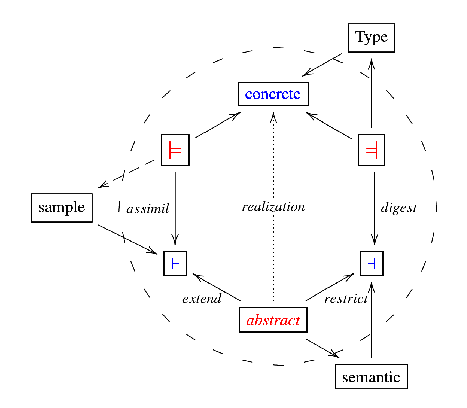
\includegraphics[]{part8/Viallefond_P52/P52_3.eps}
\\ Figure 3

 \end{center}
\end{minipage}
\hfill

A type realization is a formation rule, the yield of a judgment. Therefore, there is an arrow $\models\xrightarrow{judgment}\text{\tiny Type}$. Furthermore we may consider that an event is the arrow $\models\xleftarrow{event}=\!\!\!|$ triggered by a new sample (or exception) added to the field of knowledge. Given this interpretation there is a commutative square with a factorization where the judgment arrow is a left lifting, event a co-fibration and the arrow  $\text{Type}\rightarrow\text{concrete}$ a fibration (one of the axioms of the Model category, see also \cite{awodey_2009}). In an evolutionary system we have the arrow $\overset{}{\vdash}\xrightarrow{evolution}\overset{}{\dashv}$ and in this case we denote {\it transgression} the lifting $\overset{}{\text{\tiny semantic}}\xrightarrow{transgression}\overset{}{\vdash}$. We conclude that raising a type is a judgment in an evolution the transgression arrow which has for domain the evolution arrow and co-domain the judgment arrow. Figure~3 is very instructive. For example, using the bra-ket notation, we have \begin{displaymath}
<\!\text{Type}~|~\text{\color{blue}concrete}\!
><\!\text{\color{red}model}~|~\text{sample}\!>~ =~ 
<\!\text{Type,{\color{red}model}}~|~\text{{\color{blue}concrete},sample}\!>
\end{displaymath}
The experimentation is by essence the ket $|\text{\color{blue}concrete},\text{sample}>$. Therefore the duality 
\begin{displaymath}
<\!\text{judgment}~|~\text{experimentation}\!>,
\end{displaymath}
which subsumes the title "{\it Formal semantic to model experimental data}".

\section{The Borromean logic}
{\bf Definition} (\cite{guitart_2012}): A reduced borromean object in the category $\mathcal{C}$ with null morphisms, a terminal and initial object, cokernels and finite sums, finite coproducts, is an object $\textbf{\em {B}}$ equipped with three objects $\textbf{\em {R}}$,$\textbf{\em {S}}$,$\textbf{\em {T}}$ and an epimorphic family of monomorphisms in  $\mathcal{C}$,
\begin{displaymath}
	r\!:\!\textbf{\em {R}}\rightarrow\textbf{\em {B}},\; s\!:\!\textbf{\em {S}}\rightarrow\textbf{\em {B}},\; t\!:\!\textbf{\em {T}}\rightarrow\textbf{\em {B}}
\end{displaymath}
such that 
$\textbf{\em {B}}/r\simeq 1$,  
$\textbf{\em {B}}/s\simeq 1$,
$\textbf{\em {B}}/t\simeq 1$. In the category of finite boolean algebras this notion is equivalent to a tripartition of a set. Let exception=$\{e\}$ for R, semantic=$\{s\}$ for S, 0 the initial object and $T=1$ the constructed terminal object.

Folding the three outer triangles of Figure~3 to join in the inner part leads to
\begin{figure}[h!]
\centering
  \includegraphics[]{part8/Viallefond_P52/P52_4.eps}
  \\ Figure 4
  \end{figure}


\noindent which reveals three notions:\\
{\it 1)} {\bf conceptualisation}: $Type/abstract~ =~ concrete$ which is a {\it realization}\\
{\it 2)} {\bf analysis}: $Type/model~ =~ \dashv$ which is a {\it retrospection} and\\
{\it 3)} {\bf learning}: $Type/digestion~ =~ \vdash$ which is a {\it prospection}.\\
The retrospection and prospection being the corrolaries of the realization. Figure~4 highlights also the duality between two concepts, the pair abstraction-completude. Completude induces closure, the meaning of this circle in the diagrams.

\section{Conclusion}
The theory of the Measuremet Set (work in progress) reveals the ubiquity of a structure, a triangle encompassing a hexagon. Results presented here shows this ubiquity  now at the level of the XML-Schema grammar defining concepts. This ubiquity is bound to the  modeling activity to express the meaning of things, a conceptualization. Semantics is introduced by developing structures which have symmetries, these introducing relations are carriers of meaning.

\acknowledgements {\small I am grateful to Vivek Krishna, author of the C++ schema parser available at \url{http://wsdlpull.sourceforge.net}.  

\bibliographystyle{asp2010}
\bibliography{editor}
